\chapter{Conclusion}
brief of conclusion

\section{Conclusion of Problems}
Tell about solving the problem

\section{Conclusion of Method}
Tell about solving using method

\section{Conclusion of Experiment}
Tell about solving in the experiment

\section{Conclusion of Result}
tell about result for purpose of this research.



\section{Rahmi Roza-1164085}
\subsection{Teori}
Praktek Tugas Harian 
\begin{enumerate}

\item Mengapa Kata-Kata Harus di Vektorisasi
\par Kata harus di vektorisasi dikarenakan mesin hanya mampu membaca data dalam bentuk angka. Oleh karena itu diperlukan vektorisasi kata agar mesin mampu membaca data yang telah di vektorisasi. 
\par
\begin{itemize}
\item Gambar :
\par Penjelasan : Berdasarkan pengertian diatas, ada beberapa contoh yang bisa diterapkan. Untuk salah satu contoh dari klasifikasi data sendiri dapat diliat pada gambar berikut \ref{vekktorisasikataroza}.
\begin{figure}[!hbtp]
\centering
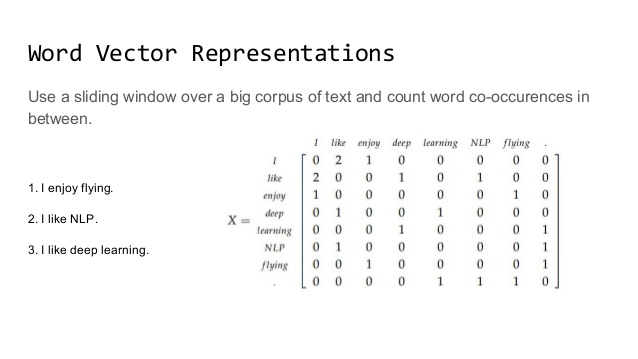
\includegraphics[scale=0.6]{figures/vekktorisasikataroza.jpg}
\caption{Vektorisasi Kata Roza}
\label{text-fadila}
\end{figure}
\end{itemize}

\item Mengapa Dimensi Dari Vektor Dataset Google Bisa Sampai 300
\par Masing-masing nilai dalam vektor 300 dimensi yang terkait dalam sebua kata "dioptimalkan" dalam  beberapa hal untuk menangkap aspek yang  berbeda dari makna dan penggunaan kata itu.Dengan kata lain masing-masing dari 300 nilai sesuai dengan beberapa fitur abstrak kata. Menghapus kombinasi nilai-nilai ini secara acak akan menghasilkan vektor yang mungkin kurang informasi penting tentang kata tersebut dan mungkin tidak lagi berfungsi sebagai representasi yang baik dari kata itu. Atau singkat cerita mungkin ada lebih dari 3 miliar kata-kata dan kalimat atau data yang tidak mungkin disimpan dalam 1 diemensi vektor makan disimpan menjadi 300 dimensi vektor untuk mengurangi kegagalan memori.
\par
\begin{itemize}
\item Gambar :
\par Penjelasan : Berdasarkan pengertian diatas, ada beberapa contoh yang bisa diterapkan. Untuk salah satu contoh dari klasifikasi data sendiri dapat diliat pada gambar berikut \ref{googleroza}.
\begin{figure}[!hbtp]
\centering
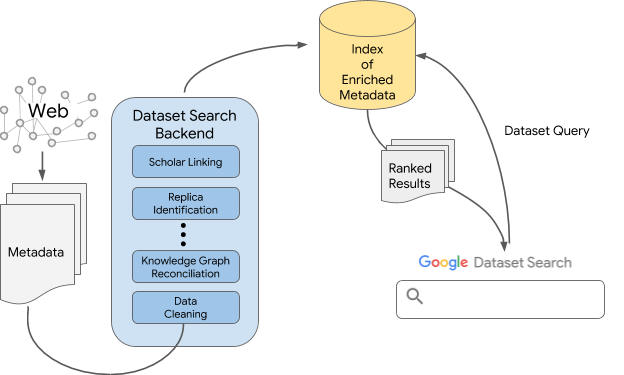
\includegraphics[scale=0.16]{figures/googleroza.png}
\caption{Google Dataset Roza}
\label{text-fadila}
\end{figure}
\end{itemize}

\item Konsep Vektorisasi Kata 
\par Konsep vektorisasi data merupakan kata-kata yang di inputkan pada mesin learning. Dan outputan nya berupa kara-kata atau keyword dari pencarian yang tekah di lakukan sebelumnya. Contoh nya pada saat kita melakukan pencarian di channel youtube kita. Maka akan muncul hasil dari pencarian dari kata-kata yang telah kita cari.
\par
\begin{itemize}
\item Gambar :
\par Penjelasan : Berdasarkan pengertian diatas, ada beberapa contoh yang bisa diterapkan. Untuk salah satu contoh dari klasifikasi data sendiri dapat diliat pada gambar berikut \ref{vekktorisasikataroza}.
\begin{figure}[!hbtp]
\centering
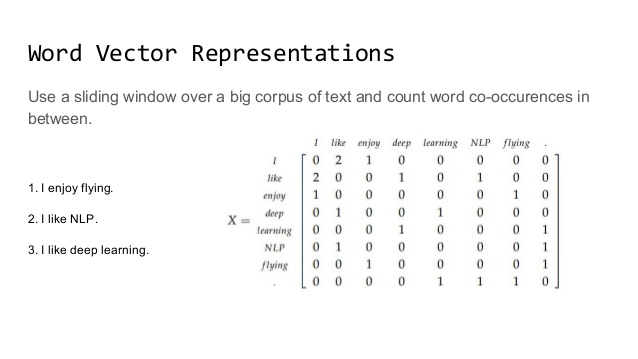
\includegraphics[scale=0.3]{figures/vekktorisasikataroza.jpg}
\caption{Vektorisasi Kata Roza}
\label{text-fadila}
\end{figure}
\end{itemize}

\item Konsep Vektorisasi Dokumen 
\par Konsep vektorisasi dokumen yaitu mesin akan membaca terlebih dahulu semua kalimat yang ada di dalam dokumen da nanti kalimat yang ada di dalam dikumen tersebut akan di oecah menjadi kata-kata.
\par
\begin{itemize}
\item Gambar :
\par Penjelasan : Berdasarkan pengertian diatas, ada beberapa contoh yang bisa diterapkan. Untuk salah satu contoh dari klasifikasi data sendiri dapat diliat pada gambar berikut \ref{vektorisasidokroza}.
\begin{figure}[!hbtp]
\centering
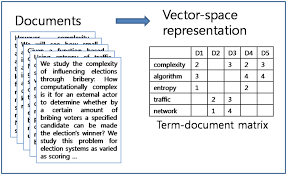
\includegraphics[scale=0.3]{figures/vektorisasidokroza.png}
\caption{Vektorisasi Dokumen Roza}
\label{text-fadila}
\end{figure}
\end{itemize}

\item Mean dan Standar Deviasi
\par Mean adalah teknik penjelasan kelompok yang didasarkan atas nilai rata-rata dari kelompok tersebut. Rata-Rata (mean) ini didapat dengan menjumlahkan data seluruh individu dalam kelompok itu, kemudian dibagi dengan jumlah individu yang ada pada kelompok tersebut. Standar deviasi adalah nilai statistik yang digunakan untuk menentukan bagaimana sebaran data dalam sampel, dan seberapa dekat titik data individu ke mean – atau rata-rata – nilai sampel.Sebuah standar deviasi dari kumpulan data sama dengan nol menunjukkan bahwa semua nilai-nilai dalam himpunan tersebut adalah sama. Sebuah nilai deviasi yang lebih besar akan memberikan makna bahwa titik data individu jauh dari nilai rata-rata.
\par
\begin{itemize}
\item Gambar :
\par Penjelasan : Berdasarkan pengertian diatas, ada beberapa contoh yang bisa diterapkan. Untuk salah satu contoh dari klasifikasi data sendiri dapat diliat pada gambar berikut \ref{meanroza}.
\begin{figure}[!hbtp]
\centering
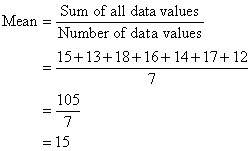
\includegraphics[scale=0.2]{figures/meanroza.png}
\caption{Mean Roza}
\label{text-fadila}
\end{figure}
\begin{figure}[!hbtp]
\centering
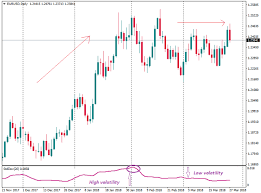
\includegraphics[scale=0.2]{figures/standarroza.png}
\caption{Standar Deviasi Roza}
\label{text-fadila}
\end{figure}
\par
\end{itemize}

\item Skip Gram
\par Skip-Gram mencoba memprediksi vektor kata-kata yang ada di konteks diberikan vektor kata tertentu. Skip-gram membuat sepasang kata target dan konteks sebagai sebuah instance sehingga skip-gram cenderung lebih baik ketika ukuran corpus sangat besar.
\par
\begin{itemize}
\item Gambar :
\par Penjelasan : Berdasarkan pengertian diatas, ada beberapa contoh yang bisa diterapkan. Untuk salah satu contoh dari klasifikasi data sendiri dapat diliat pada gambar berikut \ref{skipgramroza}.
\begin{figure}[!hbtp]
\centering
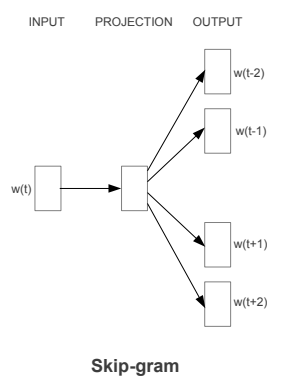
\includegraphics[scale=0.2]{figures/skipgramroza.png}
\caption{Skip-Gram Roza}
\label{text-fadila}
\end{figure}
\end{itemize}
\end{enumerate}

\begin{itemize}
\item Plagiarisme Roza
\begin{figure}[!hbtp]
\centering
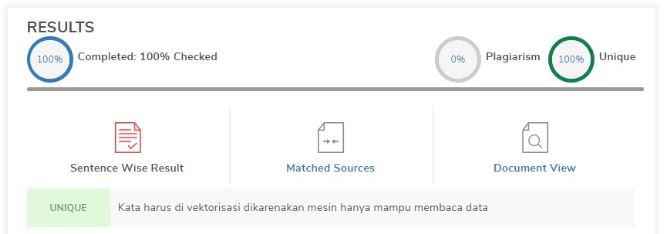
\includegraphics[scale=0.2]{figures/plagiarismeroza.jpg}
\caption{Plagiarisme Roza}
\label{text-fadila}
\end{figure}
\end{itemize}


\par
\par
\par
\par
\par
\section{Fadila-1164072}
\subsection{Teori}
Penjelasan Tugas Harian 9 ( No 1-6 ). ( No. 7 Bukti Plagiarisme )
\begin{enumerate}
\item Mengapa Kata-Kata Harus Di Lakukan Vektorisasi Dan Ilustrasi Gambar
\begin{itemize}
\item Penjelasan :
\par Alasan mengapa kata-kata harus dilakukan vektorisasi terlebih dahulu yaitu dikarenakan mesin hanya mampu membaca data dengan bentuk angka. Berdasarkan hal tersebut maka tentunya diperlukan vektorisasi kata atau bisa disebut dengan mengubah kata menjadi bentuk vektor agar mesin seolah-olah paham apa yang kita maksudkan dan dapat memproses aktifitas/perintah dengan benar. Kata juga harus di vektorisas iuntuk mengetahui presentase kata yang sering muncul dalam setiap kalimatnya, yang berguna untuk menetukan kata kunci.
\par
\item Ilustrasi Gambar
\par Penjelasan : Berdasarkan penjelasan diatas, ada beberapa contoh yang bisa diterapkan. Untuk salah satu contoh dari vektorisasi kata dapat diliat pada gambar berikut \ref{Vektorisasi Kata-fadila}.
\begin{figure}[!hbtp]
\centering
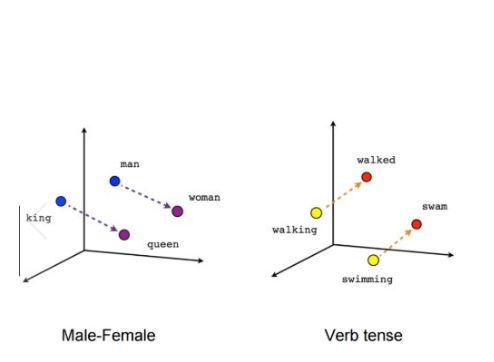
\includegraphics[scale=0.2]{figures/word-vec-fadila.jpg}
\caption{Vektorisasi Kata-fadila}
\label{Vektorisasi Kata-fadila}
\end{figure}
\par
\end{itemize}
\par
\par
\item Mengapa Dimensi Dari Vektor Dataset Google Bisa Mencapai 300 Dan Ilustrasi Serta Contoh Gambar
\begin{itemize}
\item  Penjelasan :
\par Dimensi dari Vektor Dataset Google Bisa Mencapai 300 itu dikarenakan pada masing-masing objek yang terdapat pada dataset akan memiliki identitasnya tersendiri, selain itu juga untuk nilai dalam vektor 300 dimensi yang terkait dalam sebua kata "dioptimalkan" dalam  berbagai hal untuk menangkap aspek yang berbeda dari makna dan penggunaan kata itu. secara singkatnya terdapat ada lebih dari 3 miliar kata-kata dan kalimat yang tidak mungkin disimpan dalam 1 diemensi vektor, lalu disimpan menjadi 300 dimensi vektor untuk mengatasi yang namanya kegagalan memori
\item Ilustrasi :( berdasarkan identitas tersendiri ) Apabila dicontohkan dengan penjelasan yang lebih rinci maka dilakukan perumpamaan sederhana. Misalnya untuk sebuah dataset google yang memiliki 3 buah objek yaitu berat, lebar, dan tinggi.  Kemudian dari masing-masing objek tersebut dilakukan perbandingan antara berat dan lebar beserta berat dan tinggi. Hasil yang didapatkan akan memiliki presentasi yang berbeda sehingga dapat diartikan bahwa mesin dapat membedakan objek yang hampir serupa namun tak sama.
\par 
\item Contoh Gambar
\par Penjelasan : Berdasarkan penjelasan diatas, ada beberapa contoh yang lain bisa diterapkan. Untuk salah satu contoh dari vektor dataset googlei dapat diliat pada gambar berikut \ref{Dimensi Vektor Dataset Wikipedia-fadila} dan \ref{Dimensi Vektor Dataset-fadila}.
\begin{figure}[!hbtp]
\centering
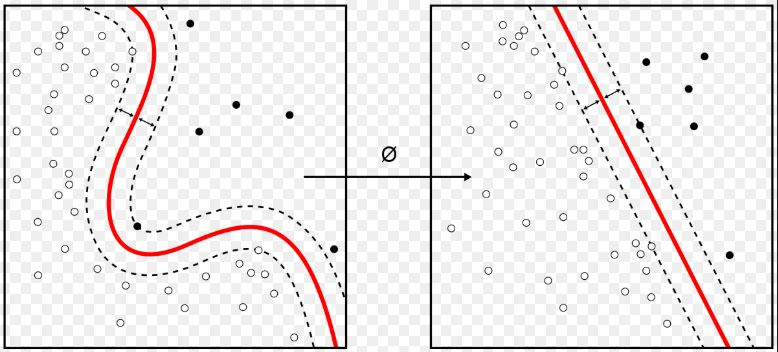
\includegraphics[scale=0.15]{figures/google-dataset-wikipedia-fadila.jpg}
\caption{Dimensi Vektor Dataset Wikipedia-fadila}
\label{Dimensi Vektor Dataset Wikipedia-fadila}
\end{figure}
\par
\begin{figure}[!hbtp]
\centering
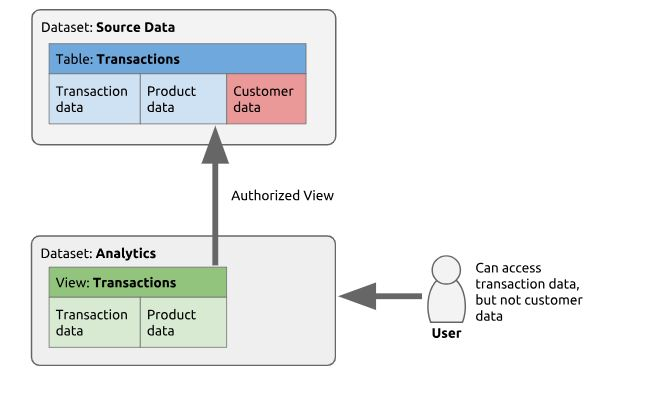
\includegraphics[scale=0.15]{figures/google-dataset-fadila.jpg}
\caption{Dimensi Vektor Dataset -fadila}
\label{Dimensi Vektor Dataset-fadila}
\end{figure}
\par
\end{itemize}
\par
\par
\item Konsep Vektorisasi Untuk Kata Dan Ilustrasi Gambar
\begin{itemize}
\item  Penjelasan :
\par Konsep untuk vektorisasi kata sebenarnya sama dengan ketika dilakukan input suatu kata pada mesin pencarian. Kemudian untuk hasilnya akan mengeluarkan ( berupa ) referensi mengenai kata tersebut. Jadi data kata tersebut didapatkan dari hasil pengolahan pada kalimat-kalimat sebelumnya yang telah diolah. Contoh sederhananya pada kalimat berikut ( Please click the alarm icon for more notifications about my channel ), pada kalimat tersebut terdapat konteks yakni channel, kata tersebut akan dijadikan data latih untuk mesin yang akan dipelajari dan diproses. Jadi ketika kita inputkan kata channel, maka mesin akan menampilkan keterkaitannya dengan kata tersebut sehingga akan lebih efisien dan lebih mudah.
\par
\item Ilustrasi Gambar
\par Penjelasan : Berdasarkan konsep diatas, ada beberapa contoh yang bisa diterapkan. Untuk salah satu contoh dari vektorisasi kata dapat diliat pada gambar berikut \ref{Vektorisasi Untuk Kata-fadila}.
\begin{figure}[!hbtp]
\centering
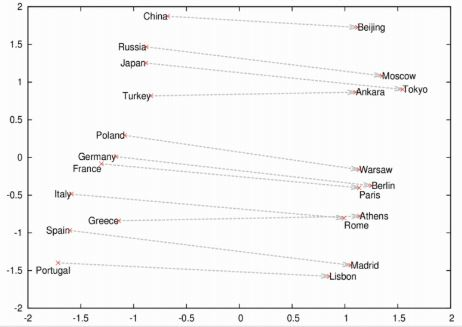
\includegraphics[scale=0.2]{figures/concept-word-fadila.jpg}
\caption{Vektorisasi Untuk Kata-fadila}
\label{Vektorisasi Untuk Kata-fadila}
\end{figure}
\par
\end{itemize}
\par
\par
\item Konsep Vektorisasi Untuk Dokumen Dan Ilustrasi Gambar
\begin{itemize}
\item  Penjelasan :
\par Untuk vektorisasi dokumen sebenarnya terbilang sama dengan konsep vektorisasi kata, yang membedakan hanya pada proses awalnya ( pada eksekusi awal ). Untuk vektorisasi dokumen ini, mesin akan membaca semua kalimat yang terdapat pada dokumen tersebut, kemudian kalimat yang terdapat pada dokumen tersebut akan di pecah menjadi kata-kata. Seperti itulah konsep vektorisasi dokumen.
\par
\item Ilustrasi Gambar
\par Penjelasan : Berdasarkan konsep diatas, ada beberapa contoh yang bisa diterapkan. Untuk salah satu contoh dari vektorisasi dokumen dapat diliat pada gambar berikut \ref{Vektorisasi Untuk Dokumen-fadila}.
\begin{figure}[!hbtp]
\centering
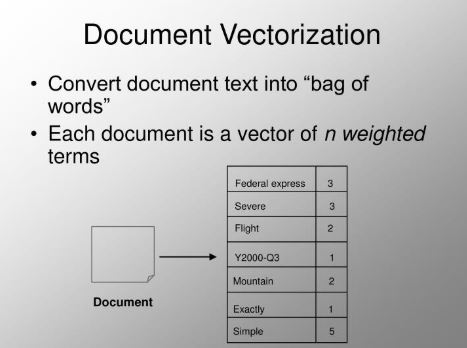
\includegraphics[scale=0.2]{figures/doc-vec-fadila.jpg}
\caption{Vektorisasi Untuk Dokumen-fadila}
\label{Vektorisasi Untuk Dokumen-fadila}
\end{figure}
\par
\end{itemize}
\par
\par
\item Pengertian Mean Dan Standar Devisiasi Beserta Ilustrasi Gambar
\begin{itemize}
\item  Pengertian Mean :
\par Mean merupakan nilai rata-rata dari suatu data. Mean sendiri dapat dicari dengan cara membagi jumlah data dengan banyak data sehingga diperoleh lah nilai rata-rata dari suatu data yang dicari / tersebut. 
\par
\par
\item  Pengertian Standar Devisiasi :
\par Untuk standar deviasi sendiri merupakan sebuah teknik statistik yang digunakan dalam menjelaskan homogenitas kelompok ataupun dapat diartikan dengan nilai statistik dimana dimanfaatkan untuk menentukan bagaimana sebaran data dalam sampel, serta seberapa dekat titik data individu ke mean atau rata-rata nilai sampel yang ada. 
\par
\par
\item Ilustrasi Gambar
\par Penjelasan : Berdasarkan penjelasan diatas, ada beberapa contoh yang bisa diterapkan. Untuk salah satu contoh dari mean dan standar devisiasi sendiri dapat diliat pada gambar berikut \ref{Mean-fadila} , \ref{Mean2-fadila}  dan \ref{Standar Devisiasi-fadila}.
\begin{figure}[!hbtp]
\centering
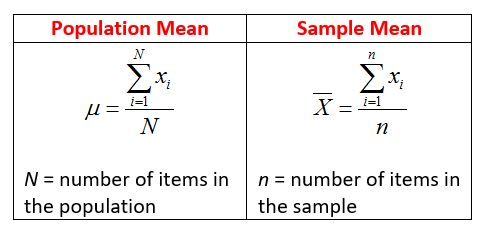
\includegraphics[scale=0.17]{figures/mean-fadila.jpg}
\caption{Mean-fadila}
\label{Mean-fadila}
\end{figure}
\par
\begin{figure}[!hbtp]
\centering
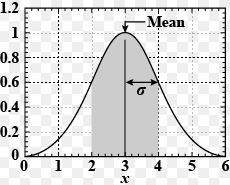
\includegraphics[scale=0.17]{figures/mean2-fadila.jpg}
\caption{Mean Lanjutan-fadila}
\label{Mean2-fadila}
\end{figure}
\par
\begin{figure}[!hbtp]
\centering
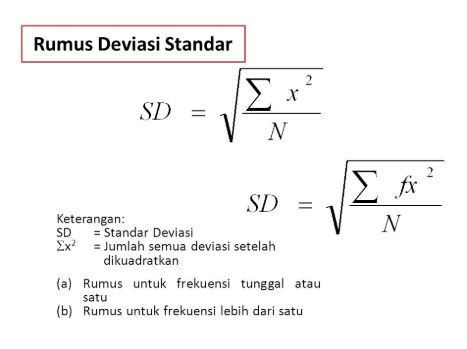
\includegraphics[scale=0.17]{figures/deviasi-fadila.jpg}
\caption{Standar Devisiasi-fadila}
\label{Standar Devisiasi-fadila}
\end{figure}
\par
\end{itemize}
\par
\par
\item Penjelasan Skip-gram Dan Ilustrasi Gambar
\begin{itemize}
\item  Penjelasan :
\par Sebuah  teknik yang digunakan di area speech processing, dimana n-gram yang dibentuk kemudian ditambahkan juga dengan tindakan “skip” pada token-tokennya. 
\par Untuk membentuk k-skip-n-grams, ada dua nilai yang harus didefinisikan, dimana kedua nilai tersebut yaitu k (jumlah kata yang di-skip) dan n (banyak kata dalam n-gram, e.g. bigram (2-gram), trigram (3-gram), dll.).
\par
\item Ilustrasi Gambar
\par Penjelasan : Berdasarkan penjelasan diatas, ada beberapa contoh yang bisa diterapkan. Untuk salah satu contoh dari skip-gram sendiri dapat diliat pada gambar-gambar berikut \ref{Plagiarisme - fadila} .
\begin{figure}[!hbtp]
\centering
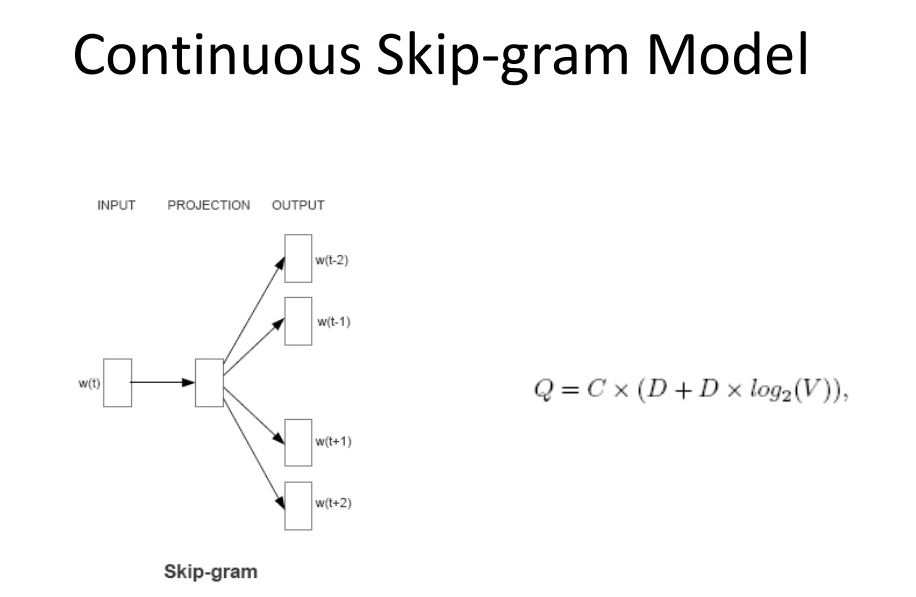
\includegraphics[scale=0.17]{figures/skip-gram-fadila.jpg}
\caption{Skip Gram - fadila}
\label{Skip Gram - fadila}
\end{figure}
\par
\par
\end{itemize}
\par
\par
\par
\par
\item Plagiarisme Fadila :
\begin{figure}[!hbtp]
\centering
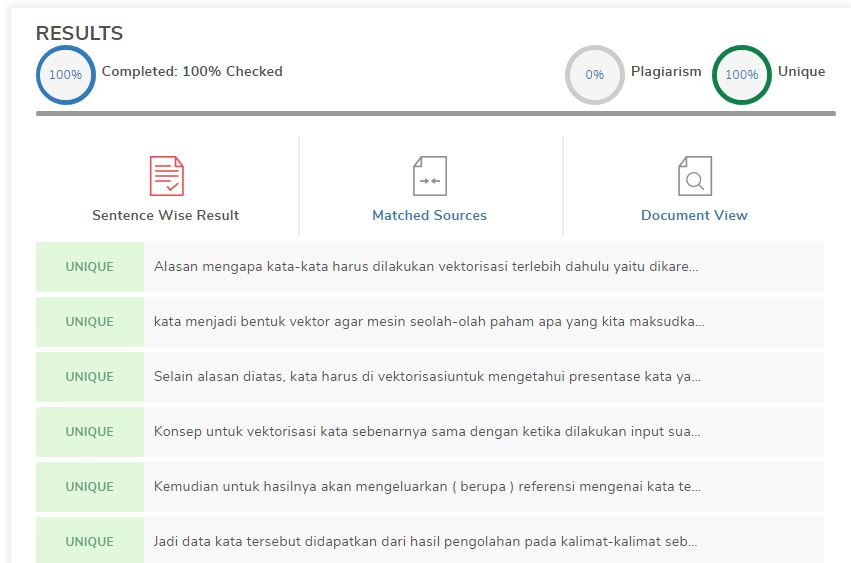
\includegraphics[scale=0.2]{figures/plagiarismm-fadila.jpg}
\caption{Plagiarisme - fadila}
\label{Plagiarisme - fadila}
\end{figure}
\end{enumerate}